
\section{Notes}

A 1-gpm
(0.06 liter/sec) side stream of the primary salt is
continuously processed to remove
 233 P a , to recover the
bred
 233 U , and to adjust the fissile content. Robertson summary
 
 Robertson does not define thorium feed rate?
 
 Serpent2 continuous reprocessing section cite own presentations at Serpent user group meetings

\section{SaltProc}

SaltProc is used in this work because it provides an accurate model of the MSBR, uses Serpent2 for transport and depletion calculations, and because it provides a batchwise reprocessing scheme which can be customized fairly easily. There are different versions of SaltProc which have slightly different methods in how the depletion data is stored as well as how reprocessing rates are calculated.

\subsection{SaltProc v0.1}

This is the first full version of SaltProc which was publicly released, and provides all the functionality necessary for modeling the MSBR with batchwise reprocessing. This version uses 3 day steps and does not perform fractional reprocessing at each step, but instead performs reprocessing according to the cycle times. For example, a 30 day cycle time would be implemented as no reprocessing during the first 27 days, then full 100\% removal of the target at the 30 day mark. This works well for reactor processes which are performed batchwise, such as adding uranium to the reactor which can be performed as a batch process. However, for approximating online reprocessing, this approach is not ideal, as it is less able to capture the frequency of the reprocessing.

For the refueling of the reactor, the thorium feed rate was set to maintain the thorium mass in the reactor. The uranium feed rate was set to be equivalent to the protactinium removal rate. Both refueling processes occur every 3 days. 

Another difference is that this version makes use of the h5py Python package to handle the hdf5 data files which contain depletion data. Within the hdf5 file, the atom density of each isotope before and after batchwise reprocessing is recorded as well as different reactor parameters such as the neutron multiplication factor.


\subsection{SaltProc v0.3}

This version of SaltProc includes an example MSBR which users can run as soon as SaltProc is installed, though some of the run parameters such as neutrons per generation and run time have to be altered to generate a more valid model. This model also uses 3 day steps, but instead of performing the batch removal only at the cycle time value, this model removes a fraction every 3 days. For example, a 30 day cycle time would result in 10\% removal every 3 days. This more accurately models online reprocessing, which is primarily what the MSBR employs in its reprocessing scheme aside from the salt discard.

The reactor refueling is performed slightly differently from v0.1 as well. This version assumes a constant ratio between the uranium refueling and the thorium refueling. The net refueling for each 3 day depletion step is set to maintain the mass of the system.

Additionally, this version of SaltProc uses the PyTables Python package for handling the hdf5 data files. The data files are structured similarly to v0.1 of SaltProc, but instead of atom density they use mass, which makes analysis of the files slightly more user friendly.

\section{Serpent2 Continuous Reprocessing}

The continuous reprocessing functionality of Serpent2 was undocumented for several years aside from on the Serpent2 forums, but more recently work has gone into providing documentation. However, there has not been comparisons of Serpent2 continuous reprocessing with Serpent2 batchwise reprocessing with no differences between the models aside from the mathematical reprocessing approach used.

As discussed in the documentation work of the continuous reprocessing functionality, there are three different options which can be used for the Serpent2 built-in continuous reprocessing. The different options are 0, 1, and 2; which are henceforth referenced as Constant, Decay, and Step reprocessing.

\subsection{Constant}
The Constant reprocessing method is the only method of the three options which does not conserve mass. This option instead generates mass the same way as the Decay reprocessing method for the initial step, then continues using that mass rate from that point onwards.

The main issue with this method is that it, for Serpent 2.32.1, it causes depletion to cease functioning while this method is active. This is an issue, since for most cases where a user wants to incorporate a feed rate, depletion is being considered.

\subsection{Decay}
The Decay reprocessing method is the most useful of the three options, and that is due to its flexibility in its usefulness. This method adds a decay term to whatever material it is attached to, and that decay term becomes a feed term to whatever material is set to receive the flow. For fission product removal, this is likely some material which is not modeled in the geometry of the problem but only exists to receive the fission product waste. However, this term can instead be leveraged to turn it into a feed rate.

This can be performed by attaching the decay term to a material which contains a volume of the desired feed, and then having that material feed into the core. The feed then "decays" from the feed tank into the core, essentially operating as a feed. Using this same method but altering the reprocessing constant or volume of the feed tank allows for an essentially constant feed rate, where the removed mass is negligible compared to the net mass.

Additionally, for this method, there are multiple approaches which can be used to calculate the reprocessing constants that should be implemented. These approaches are named "Cycle Time Decay", "Cycle Rate", and "SaltProc Cycle Rate" accordingly. The Cycle Time Decay approach treats the cycle time as if it is twice a half-life, and the cycle time is an exponential process. The Cycle Rate approach treats the cycle time as the time where 100\% of removal occurs, and then linearly extrapolates by assuming an equal percentage removal occurs up to that point.

The reason these approaches are implemented is because molten salt reactor reprocessing schemes provide reprocessing data in terms of cycle times. The cycle time is the amount of time it takes for a given element to be removed from the system. This cannot be directly solved using the Bateman equation, as shown in Equations \eqref{eq:decay_1} through \eqref{eq:decay_3} and \eqref{eq:decay_4} through \eqref{eq:decay_7}. 

\begin{equation} \hfill
\frac{dN}{dt} = -\lambda_r N
\hfill\label{eq:decay_1} \end{equation}

\begin{equation} \hfill
N(\tau) = 0 = N_0 e^{-\lambda_r \tau}
\hfill\label{eq:decay_2} \end{equation}

\begin{equation} \hfill
-ln(0) = \lambda_r \tau
\hfill\label{eq:decay_3} \end{equation}

Equations \eqref{eq:decay_1} through \eqref{eq:decay_3} show how the solution results in a reprocessing constant of infinity when only continuous removal is considered.

\begin{equation} \hfill
\frac{dN}{dt} = C -\lambda_r N
\hfill\label{eq:decay_4} \end{equation}

\begin{equation} \hfill
N(\tau) = 0 = N_0 e^{-\lambda_r \tau} + \frac{C}{\lambda_r} \left( 1 - e^{-\lambda_r \tau} \right)
\hfill\label{eq:decay_5} \end{equation}

\begin{equation} \hfill
0 = N_0 e^{-\lambda_r \tau} + \frac{C}{\lambda_r} - \frac{C}{\lambda_r} e^{-\lambda_r \tau}
\hfill\label{eq:decay_6} \end{equation}

\begin{equation} \hfill
0 = \lambda_r N_0 e^{-\lambda_r \tau} + C - C e^{-\lambda_r \tau}
\hfill\label{eq:decay_7} \end{equation}


 Equations \eqref{eq:decay_4} through \eqref{eq:decay_7} show that the only real solution to a steady accumulation and continuous removal is with a reprocessing constant of 0. 

\subsubsection{Cycle Time Decay}

The Cycle Time Decay approach is a simple method which makes use of the mathematical form of the Decay reprocessing method. Because it adds a "decay-like" term to the Bateman equation, this approach takes the cycle time for the target, cuts it in half, and then treats that value as the reprocessing half-life for that target. This process is shown in Equations \eqref{eq:ctd_1} and \eqref{eq:ctd_2}.

\begin{equation} \hfill
\tau_{1/2} = \frac{T_{cyc}}{2}
\hfill\label{eq:ctd_1} \end{equation}

\begin{equation} \hfill
\lambda_r = \frac{ln(2)}{\tau_{1/2}}
\hfill\label{eq:ctd_2} \end{equation}

An example of how this approach is mathematically modeled can be seen in Figure \ref{fig:ctd_examp}.

\begin{figure}[H]
  \centering
  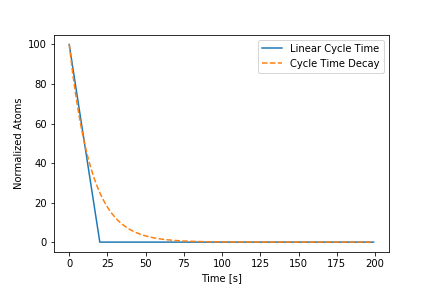
\includegraphics[scale=0.6]{images/Cycle_Time_Decay_example_0.png}
  \caption{A comparison between a linear 20 second cycle time and the Cycle Time Decay approach.}
   \label{fig:ctd_examp}
\end{figure}

It can be seen in this figure that this approach is accurate in being close to the cycle time, though this accuracy is limited to above approximately 40\% of the atoms. Because fission products are continuously generated though, it is expected to be within the more accurate regions.
%Figure \ref{fig:ctd_examples} shows how the Cycle Time Decay approach fares when accumulation of fission products is incorporated into the problem. 

%\begin{figure}[H]
%  \centering
%  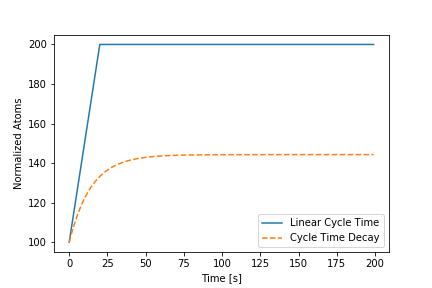
\includegraphics[scale=0.6]{images/Cycle_Time_Decay_example_10.png}
%  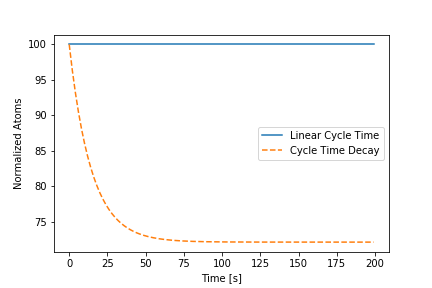
\includegraphics[scale=0.6]{images/Cycle_Time_Decay_example_5.png}
%  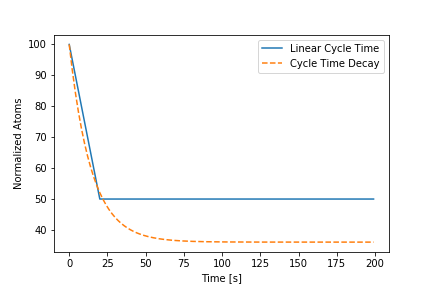
\includegraphics[scale=0.6]{images/Cycle_Time_Decay_example_2.5.png}
%  \caption{Comparison with linear 20 second cycle time and Cycle Time Decay approach for 10, 5, and 2.5 %atoms per second accumulation, respectively.}
%   \label{fig:ctd_examples}
%\end{figure}

%The top plot of Figure \ref{fig:ctd_examples} shows a situation where the accumulation of fission products occurs at a higher rate than the cycle time, leading to a larger steady-state value than initially present. The Cycle Time Decay does not reach the 200 value and instead is lower at 144. The middle plot shows a situation where the accumulation rate matches the cycle time removal rate, the same rate that the linear cycle time would have them removed, resulting in a steady-state value. However, the Cycle Time Decay approach drops to approximately 72 levels off. The bottom plot shows an accumulation which is half the linear cycle time removal rate. These results are somewhat close, though the Cycle Time Decay does not reach the same steady-state value, instead stabilizing around 40 instead of 50. For various accumulation rates ranging from 0.1 to 1 million atoms per second, the steady-state difference comes out to approximately 27.86\% for each. This percent difference also stays the same for different cycle times as well.

An example of implementing this approach for a 30 second cycle time would then have a 15 second reprocessing half-life. This is then converted to a reprocessing constant in the same way that a decay half-life is converted to a decay constant, which can be seen in Equation \eqref{eq:ctd_eqn}, resulting in a value of 0.0462 $s^{-1}$.

\begin{equation} \hfill
\lambda_{r} = \frac{ln(2)}{15} = 0.0462 s^{-1}
\hfill\label{eq:ctd_eqn} \end{equation}

\subsubsection{SaltProc Cycle Time Decay}

This approach is the same as Cycle Time Decay, but alters for any target which has a cycle time less than the batchwise reprocessing step incorporated by SaltProc. For example, a 3 day cycle time for some target would be treated the same as the standard Cycle Time Decay. However, a cycle time shorter than the 3 day batchwise reprocessing step used by SaltProc for the MSBR has its half-life extended to the SaltProc minimum value of 1.5 days. For example, a 30 second cycle time would instead be treated as a 3 day cycle time, which would result in a half-life of 1.5 days. Plugging in, this would result in a reprocessing constant of 0.462 $days^{-1}$, or 5.348E-6 $s^{-1}$. This is the reprocessing constant for any cycle time which is less than or equal to three days. 

\subsubsection{Cycle Rate}

The Cycle Rate approach uses a linear approximation such that the inverse of the cycle time is the rate at which material is removed. This is represented by, for example, 10\% removal per second would neglect the efficiency decrease over time and give 100\% removal after 10 seconds. This can be seen in Equations EQUATION.



However, the mathematical model actually results in exponential decay in the removal effectiveness due to a decreasing amount of the target to remove. Figure \ref{fig:cr_examp} shows how this approach compares to the actual exponential decay.

\begin{figure}[H]
  \centering
  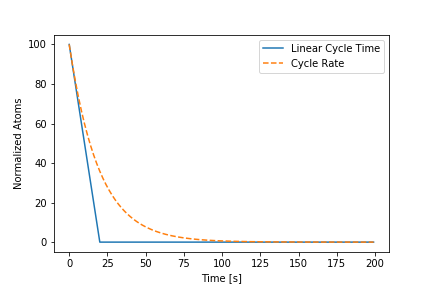
\includegraphics[scale=0.6]{images/Cycle_Rate_example_0.png}
  \caption{A comparison between a linear 20 second cycle time and the Cycle Rate approach.}
   \label{fig:cr_examp}
\end{figure}

It can be seen from this figure that the Cycle Rate approach removes at a rate sufficient to match the cycle time of 20 seconds while there are ~60\% of the atoms present. Once the atom count drops, the removal becomes less effective however, which is physical but makes the model less effective at matching the cycle time. Because the Cycle Rate approach is used on fission products which are being constantly generated, the difference is expected to be fairly small.

\begin{figure}[H]
  \centering
  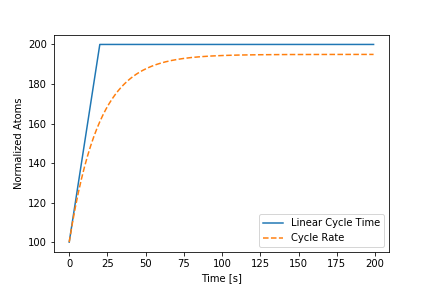
\includegraphics[scale=0.6]{images/Cycle_Rate_example_10.png}
  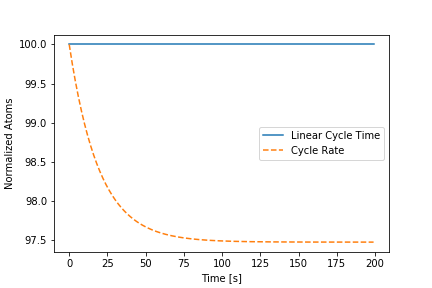
\includegraphics[scale=0.6]{images/Cycle_Rate_example_5.png}
  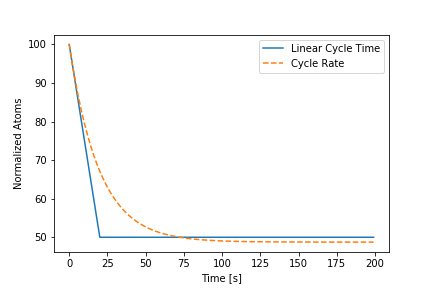
\includegraphics[scale=0.6]{images/Cycle_Rate_example_2_5.png}
  \caption{Comparison with linear 20 second cycle time and Cycle Rate approach for 10, 5, and 2.5 atoms per second accumulation, respectively.}
   \label{fig:cr_examples}
\end{figure}



An example cycle time of 30 seconds would be modeled by taking the inverse, which gives 0.033 $s^{-1}$. This value is then converted to a reprocessing constant by plugging it into the solved differential equation form shown in Equation \eqref{eq:ctd_eqn}, giving a value of 0.0339 $s^{-1}$.

\begin{equation} \hfill
\lambda_{r} = ln\left(\frac{1}{1 - X}\right)
\hfill\label{eq:cr_eqn} \end{equation}

The reason this approach is used is two-fold. Firstly, SaltProc v0.3 uses the same approximation for its batchwise removal, so this same method is employed to better compare the two models. Secondly, due to the mathematical nature of the Decay reprocessing model, 100\% removal only occurs for a reprocessing constant of infinity. This means an approximation must be made. This is also a reasonable approximation since there is constant addition of material, meaning that the exponential line and the linear line are not going to be significantly different.


\subsubsection{SaltProc Cycle Rate}

The SaltProc Cycle Rate approach is the same as the Cycle Rate approach, but takes into account the limiting nature of the 3 day batchwise reprocessing step used by SaltProc. For example, a 6 day cycle time target would be modeled the same using the SaltProc Cycle Rate approach as the standard Cycle Rate approach. However, anything shorter than 3 days would be modeled differently, since that is the batchwise reprocessing step inocorporated by SaltProc for modeling the MSBR. For example, a 30 second cycle time would be analyzed instead as a 3 day cycle time, since SaltProc can only remove 100\% of material after a minimum of 3 days. This means the inverse would be 0.333 $days^{-1}$, or 3.858E-4 $s^{-1}$. Converting to a reprocessing constant gives a value of 3.858E-6 $s^{-1}$. This is the reprocessing constant for any cycle time which is less than or equal to three days.

\subsubsection{Direct Linear Approach}

Another approach which is not implemented in this work is to directly apply the Cycle Rate removal rate, which is the inverse of the cycle time, as the reprocessing constant. This approach is referred to as the Direct Linear approach, and it is not implemented here because it is a flawed implementation of reprocessing. This can be seen in Table \ref{tab:repr_decay_view}, where for longer cycle times, the impact is negligible, but for shorter cycle times, the difference becomes larger.

\begin{table}[H]
\renewcommand{\arraystretch}{1.25}
\caption{Decay Reprocessing Approaches}
\label{tab:repr_decay_view}
\begin{center}
\begin{tabular}{ | c | c | c | c | }
 \hline
 Approach & Cycle Time & Removal Rate [$s^{-1}$] & $\lambda_{r}$ [$s^{-1}$]\\
 \hline
 \hline
 CR & 3 d & 3.86E-6 & 3.86E-6\\
 DL & 3 d & 3.86E-6 & 3.86E-6\\
 CR & 20 s & 0.05 & 5.13E-2\\
 DL & 20 s & 0.05 & 5.00E-2\\
 CR & 5 s & 0.2 & 2.23E-1\\
 DL & 5 s & 0.2 & 2.00E-1\\
 \hline
\end{tabular}
\end{center}
\end{table}

Figure \ref{fig:dl_cr_compare_linear} shows the implementation of both methods for an example nuclide with a cycle time of CYCLE TIME and an accumulation rate of ACCUMULATION RATE. It can be seen from this figure how the Direct Linear and Cycle Rate approaches differ in modeling of the same isotope.

\begin{figure}[H]
  \centering
  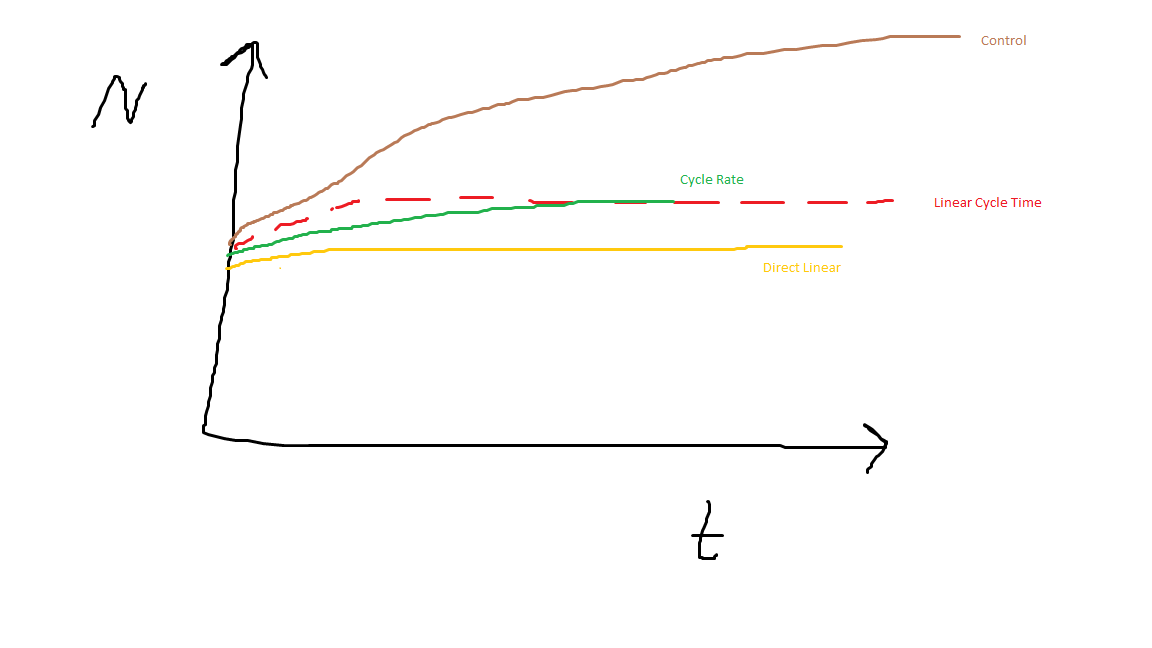
\includegraphics[scale=0.25]{images/direct_linear_compare.png}
  \caption{A comparison of the Direct Linear and Cycle Rate approaches for a particular element with a given accumulation rate and cycle time.}
   \label{fig:dl_cr_compare_linear}
\end{figure}


Figure \ref{fig:dl_cr_compare} shows how the reprocessing constants vary over different cycle times for the Direct Linear and Cycle Rate approaches. It can be seen in the figure that the main differences occur at small cycle times and the difference becomes negligible for larger cycle times.

\begin{figure}[H]
  \centering
  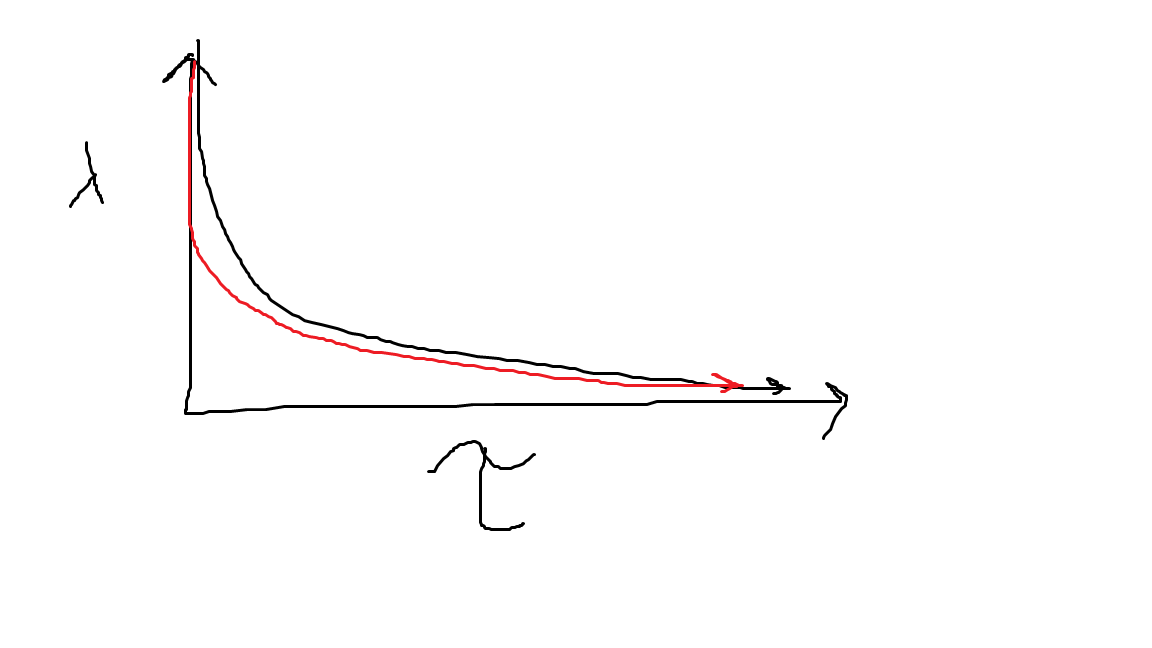
\includegraphics[scale=0.25]{images/direct_exp_compare.png}
  \caption{Comparison of the Direct Linear and Cycle Rate approaches for various cycle times and the resulting reprocessing constants.}
   \label{fig:dl_cr_compare}
\end{figure}


REFERNCE PAPER THAT USES THIS APPROACH

SHOW MATHEMATICAL ISSUE

MOVE THIS SECTION INTO LIT REVIEW

\subsubsection{Decay Approaches Summary}

Figure \ref{fig:repr_cnst} shows how the reprocessing constants for the different approaches vary as a function of cycle time.

\begin{figure}[H]
  \centering
  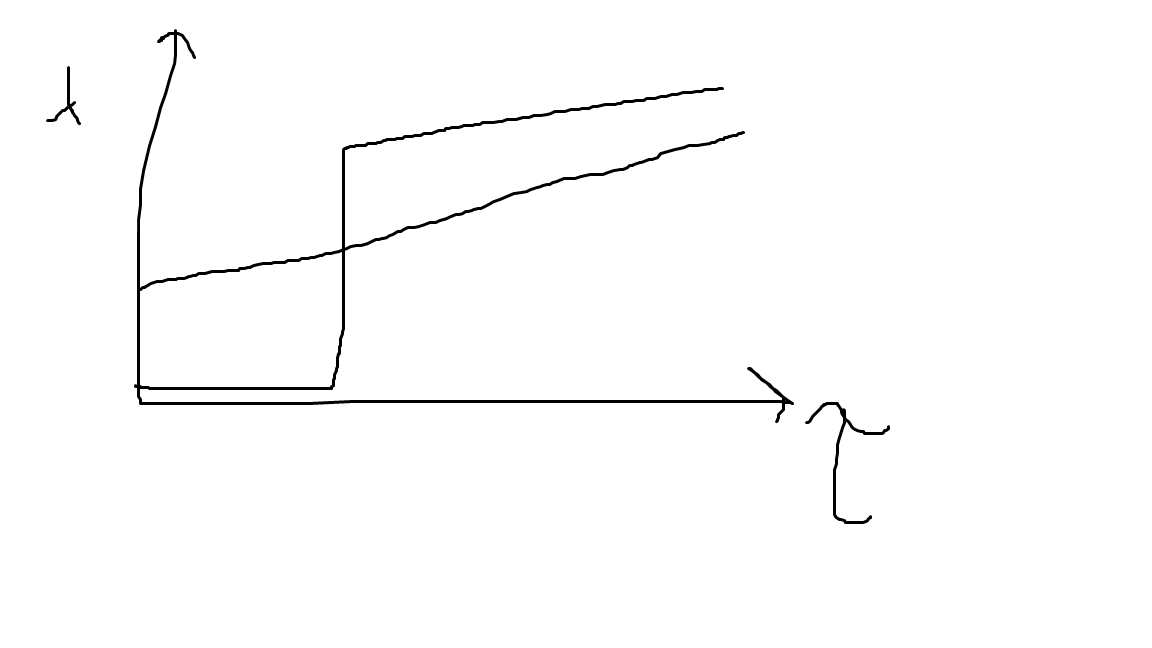
\includegraphics[scale=0.45]{images/repr_cnst_cycle.png}
  \caption{Plot of how reprocessing constants for different approaches vary with cycle time.}
   \label{fig:repr_cnst}
\end{figure}

WHICH IS THE MORE ACCURATE APPROACH BETWEEN THE TWO?

PLOT OF ACCURACY OF EACH APPROACH IN BEING MORE SIMILAR TO LINEAR/EXPONENTIAL CYCLE TIME? TRY AND FIND SOURCES ON CYCLE TIME.

CITE "The EQL0D fuel cycle procedure and its application to the transition to
equilibrium of selected molten salt reactor designs": This paper uses $\lambda = \frac{1}{T_{cycle}}$

CITE "Liquid Fuel Molten Salt Reactors for Thorium
Utilization" This paper uses bulk batchwise reprocessing

INCLUDE PLOT OF N(t) FOR DIFFERENT CYCLE TIMES WHERE ONLY INITIAL MASS AND REPROCESSING ARE CONSIDERED. (DIRECT LINEAR AND CYCLE RATE ARE THE SAME FOR LARGE CYCLE TIMES)

REPLICATE ATOMS OVER TIME PLOTS FOR DIFFERENT MODELS AND DIFFERENT ACCUMULATION RATES TO SEE HOW STEADY-STATE VALUES COMPARE

\subsection{Step}

The Step reprocessing method implemented in Serpent2 is mathematically very similar to the Decay model, but instead of updating continuously in time, it instead is updated during new depletion steps. In this manner, it is a sort of mix between the Constant method and the Decay method. This is because over a single depletion step, it is a constant added or subtracted from the Bateman equation, while over many depletion steps, it follows the same exponential decay form of the Decay method.

This particular method is not useful for extracting fission products, and is not needed for constant feed rates since that can be modeled using the Decay method. This method could be useful for inducing a step drop in feed rate, though this would require running only a single depletion step until the drop occurred. Additionally, this drop could be simulated by running the Decay method and reducing the reprocessing constant. This would allow for flexibility in the distribution of depletion steps as well without having to worry about changing the behaviour of the reprocessing functionality. 

Another potential issue with the Step method is that the depletion step can last long enough that the constant mass removal causes the mass to go negative. However, Serpent2 will cease running if this occurs. The Decay method does not mathematically allow for negative mass, the Constant method does not conserve mass, and the Step method stops running once there is negative mass.

The main potential use of the Step reprocessing may be for movement of material at a set rate. This could be implemented by writing a script to check the current number of atoms of the target and adjusting the reprocessing rate accordingly. However, for the MSBR, this form of reprocessing is not necessary, and is thus not implemented.

\section{Mass Balancing}

DIFFERENT FEED RATE VARIANTS IMPLEMENTED

MSBR MASS BALANCE BATCH AND CONTINUOUS

DENSITY CHANGE IN SERPENT2 EFFECTS

WORST CASE MASS BALANCING

\section{Convergence}

SHANNON ENTROPY

STOCHASTIC ERROR VS ACTUAL DIFFERENCE IN RESULTS

DEPLETION ERROR BUILDUP

\section{Continuous Reprocessing Implementation}

\section{Effects of Delayed Neutrons on Depletion}

PLOT OF SPECTRUMS WITH AND WITHOUT DELAYED NEUTRONS

TABLE OF IMPORTANT ISOTOPE CONCENTRATIONS FOR WITH AND WITHOUT

INCLUDE MODEL WITH SPATIAL VARIANCE IN DNPS VS NO SPATIAL VARIANCE


